\section{Rules Generation} \label{sec:rules_gen}
We introduce \krd, a disk-based approach to discover first-order Horn Rules in RDF KBs. The first task \krd needs to address is the generation of the universe of all possible rules $R$. Each rule in $R$ must cover one or more examples of the generation set $G$.

In this setting, the universe of all possible rules can be generated by just inspecting elements of $G$. In fact, a rule that does not cover any element of $G$ will never be part of the optimal solution, since it will not give any contribution to the set cover problem. This is a key part of our generation approach: we do not inspect the entire KB, but just entities belonging to $G$. The smaller the size of $G$ is, the smaller is the search space for rules generation. On the contrary, recent KB rule mining approaches tackle the problem by searching for valid rules over the entirety of the KB. This is typically done by initially looking at all facts that share a common predicate, and then expanding these facts with other predicates that share common entities~\cite{galarraga2015fast} (TODO : CITE Ontological path finding). Alternatively other approaches leverage on well established relational database techniques such as functional dependencies discovery (TODO: cite SIGMOD DEMO Data Lakes). 

The generation problem is simple but presents significant scalability issues. The number of all possible rules increases exponentially with the size of the KB and enumerating all of them means exploring a huge search space. This is the main reason why previous approaches solve the problem by loading the entire KB into main memory and by aggresively indexing triples on subject, object, and predicate. Unfortunately, modern KBs can easily exceed the size of hundreds of GBs, making a memory-based solution unfeasible on common machines. We introduce in \krd a novel rules generation technique that inspects only a portion of the KB. On the one hand, we load into main memory only a small fraction of the database. On the other hand, this model allows the extension of the language to be more expressive than previous works. One could argue that reducing the search space may lead to missing some meaningful rules. We will show in Section~\ref{sec:krd_comparative} that our generation technique for $G$ creates a representative (reduced) view of the entire search space.

\begin{figure}[t]
	\centering
	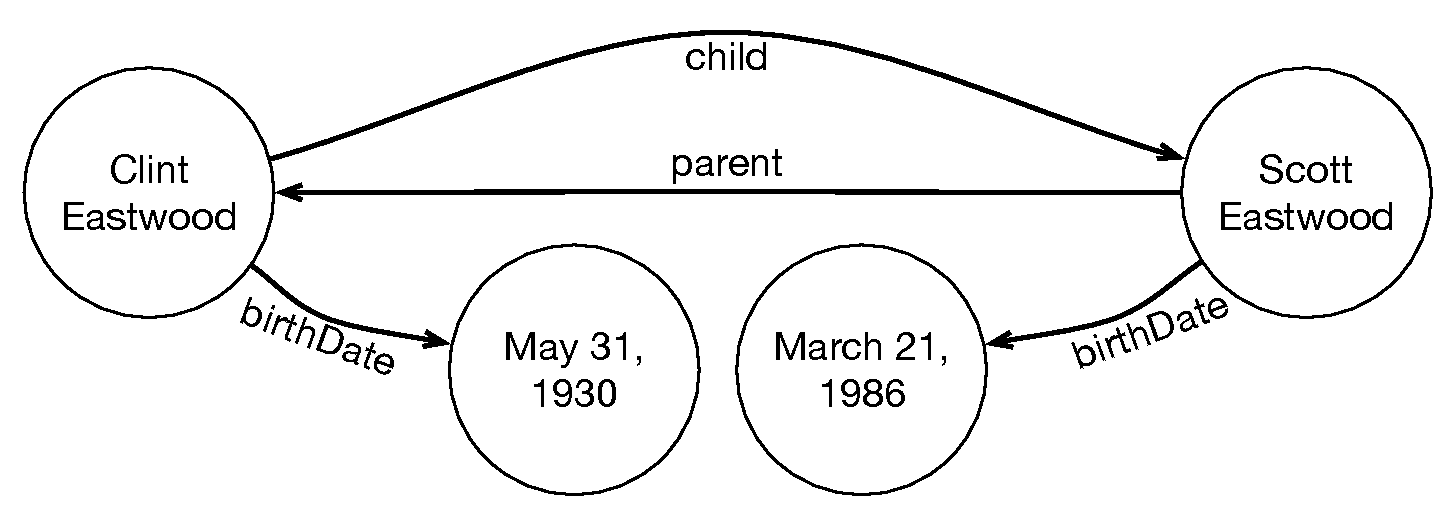
\includegraphics[width=0.6\columnwidth]{include/figure/graph_example.pdf}
	\caption{Graph Portion of \dbpedia}
	\label{fig:krd_graph_example}
\end{figure}

The data structure \krd leverages on is a straightforward translation of a KB $\kb$ into a directed graph: entities and literals are nodes of the graph, while there is a direct edge from node $a$ to node $b$ for each triple $\<a,rel,b\> \in \kb$. Edges are labelled, where the label is the relation $rel$ that connects subject to object in the triple. Figure~\ref{fig:krd_graph_example} shows a portion of \dbpedia~\cite{bizer2009dbpedia} that connects two person in a child and parent relationship, along with their dates of birth. The graph represents information of four KB triples (two birth dates, one parent and one child relation).

The body of a Horn Rule can be seen as a path in the graph. W.r.t. Figure~\ref{fig:krd_graph_example}, the body $\atom{child}{a}{b} \wedge \atom{parent}{b}{a}$ corresponds to the path \textit{Clint Eastwood} $\rightarrow$ \textit{Scott Eastwood} $\rightarrow$ \textit{Clint Eastwood}. In Section~\ref{sec:krd_language} we defined valid rules. A valid body of a rule contains target variables $a$ and $b$ at least once, and every other variable at least twice. In a valid body also each atom is transitively connected to every other atom. 
If we allow navigation of edges in any direction (no matter what the direction of the edge is on the graph), we can easily translate bodies of valid rules to valid paths on the graph.
Given a pair of entities $(x,y)$, a valid body corresponds to a valid path $p$ on the graph that meets the following criteria:
\begin{enumerate}
	\item $p$ starts at the node $x$;
	\item $p$ touches $y$ at least once;
	\item $p$ ends in $x$, in $y$, or in a different node that has been touched before.
\end{enumerate}
In other words, given the body of a rule $r_{body}$, $r_{body}$ covers a pair of entities $(x,y)$ iff there exists a valid path on the graph that corresponds to $r_{body}$. Therefore, given a pair of entities $(x,y)$, we can generate bodies of all possible valid rules by simply computing all valid paths from $x$ with a standard BFS. Note how the transitively connection between atoms is always guaranteed by the construction property of a path $p$: for each node $n$ in $p$ there always exists a subpath that connects $n$ to every other node in $p$. The key point is the ability of navigating each edge in any direction, which basically means turning the original directed graph into an undirected one.

Despite the navigation over an undirected graph, we still need to keep track of the original direction of the edges. This is essential when translating paths to Horn Rule bodies. In fact, if we navigate an edge \texttt{rel} between $a$ and $b$, an original edge direction from $a$ to $b$ produces the atom $\atom{rel}{a}{b}$, while a direction from $b$ to $a$ produces the atom $\atom{rel}{b}{a}$. These two atoms are different, where the position of variables is determined by the original direction of the edge.

One should notice that for two entities $x$ and $y$, there might exist infinite valid paths starting from $x$ since every node can be traversed multiple times. Thus we introduce the $maxPathLen$ parameter that determines the maximum number of edges in the path. When translating paths to Horn Rules, $maxPathLen$ determines the maximum number of atoms that we can have in the body of the rule. This parameter is essential to avoid the discovery of rules with infinite body length.

The main advantage of inspecting just the generation set $G$ is the capability of loading only a small portion of the graph that is currently needed. Given a pair of entities $(x,y)$, we retrieve from the  KB all those nodes at distance $maxPathLen-1$ or less from $x$ or $y$, along with their edges. Retrieving such nodes and edges can be done recursively: we maintain a queue of entities, and for each entity in the queue we fire a SPARQL query against the KB to get all entities (and edges) at distance $1$ from the current entity -- we call these queries \emph{single hop queries}. We then add the new found entities to the queue iff they are at distance less than  $maxPathLen-1$ from either $x$ or $y$ and they have not been visited before. The queue is initialised with $x$ and $y$. By doing so we retrieve a small portion of the entire KB, the only one needed to discover rules that cover $(x,y)$. We will show in the experimental section that SPARQL engines are very fast at executing single hop queries.

The generation of the universe of all possible rules for $G$ is then straightforward: for each element $(x,y) \in G$, we construct the portion of the graph as described above and compute all valid paths starting from $x$. Computing paths for every example in $G$ implies also computing the coverage over $G$ for each rule. The coverage of a rule $r$ is simply the number of elements in $G$ where there exists a path that corresponds to $r_{body}$. Our discovery technique will also generate single-instance rules: rules that cover only one example $(x,y) \in G$ by instantiating target variables $a$ and $b$ in the rule with $x$ and $y$. Once the universe of all possible rules has been generated (along with coverages over $G$), computing coverage and unbounded coverage over $V$ is just a matter of executing two SPARQL queries against the KB for each rule in the universe. 
We will show in Section~\ref{sec:krd_greedy} how some queries can be avoided, as well as there is no need of enumerating all possible rules in the universe as some of them will never be part of the final solution.

Clearly, the size of $G$ has a direct impact on the search space and hence on the running time. Since we generate all valid rules for each example in $G$, the search space grows roughly linearly with the size of $G$. If we could know a-priori the minimum subset of examples that lead to the generation of all valid rules, then we could use only those few examples. 
%
A future direction we are working on exploits exactly this point: how to select a small number of representative examples in order to reduce the size of $G$, without significantly affecting the quality of the output.

\subsection{Input Examples Generation} \label{sec:ex_generation}
A crucial role in our approach is played by the two input sets $G$ and $V$, used to generate and validate rules. We will show that discovering negative rules is the dual problem of discovering positive rules, therefore we assume to be in the setting of generating positive rules.
We will explain how to switch to the negative setting at the end of this section.

Given an input KB $\kb$ and a predicate $rel \in \kb$, we automatically build a generation set $G$ and a validation set $V$ as follows. $G$ consists of positive examples for the target predicate $rel$. It is generated as all pairs of entities $(x,y)$ such that $\<x,rel,y\> \in \kb$ -- if the target predicate is \texttt{child}, it consists of all pairs of entities in a child relation.
$V$ instead consists of counter (negative) examples for the target predicate and it is slightly more complicated to generate, since the closed world assumption does not longer hold in KBs. Differently from classic database scenarios, we cannot assume that what is not stated in a KB is false (closed world assumption). Because of large incompleteness, everything that is not stated in a KB is $unknown$ rather false. In order to generate negative examples, we make use of a popular technique for KBs: \emph{Local-Closed World Assumption} (\emph{LCWA})~\cite{dong2014knowledge,galarraga2015fast}. LCWA states that if a KB contains one or more object values for a given subject and predicate, then it contains all possible values (if a KB contains one or more children of Clint Eastwood, then it contains all possible children). This is definitely true for \emph{functional} predicates (predicates such as \texttt{capital} where the subject can have at most one object value), while it might not hold for non-functional predicates (e.g., \texttt{child}). KBs contain many non-functional predicates, we therefore extend the definition of LCWA by considering the dual aspect: if a KB contains one or more subject values for a given object and predicate, then it contains all possible values. 

To generate negative examples we then take the union of the two LCWA aspects: for a given predicate $rel$, a negative example is a pair $(x,y)$ where either $x$ is the subject of one or more triples $\<x,rel,y'\>$ with $y \neq y'$, or $y$ is the object of one or more triples $\<x',rel,y\>$ with $x \neq x'$. As an example, if $rel=\texttt{child}$, a negative example is a pair $(x,y)$ such that $x$ has some children in the KB that are not $y$, or $y$ is the child of someone that is not $x$. By considering the union of the two LCWA aspects we do not restrict predicates to be functional (such as in~\cite{galarraga2015fast}). 

The number of negative examples generated with the above technique could easily explode (for a target \texttt{child} predicate it is nearly the cartesian product of all the people having a child with all the people having a parent). In order to apply the same approach for positive and negative rules discovery, we require $G$ and $V$ to be of comparable sizes. We therefore introduce a further constraint, that significantly shrinks the size of negative examples: given a pair of entities $(x,y)$, $x$ must be connected to $y$ via a predicate that is different from the target predicate. In other words, given a Kb $\kb$ and a target predicate $rel$, $(x,y)$ is a negative examples if $\<x,rel',y\> \in \kb$, with $rel' \neq rel$. This intuition exploits the LCWA for predicates rather than for entities. If a KB contains a relation between two entities $x$ and $y$, then it contains all possible relations between $x$ and $y$. If $x$ and $y$ are in a relation that is not the target predicate, then most likely $x$ and $y$ are not connect by the target predicate in the real world. This further restriction has multiple advantages: on the one hand it makes the size of $V$ of the same order of magnitude of $G$ (see Section~\ref{sec:krd_experiments}), on the other hand it guarantees the existence of a path between $x$ and $y$, for every $(x,y) \in V$. For positive examples, the existence of a path was already guaranteed since pairs in $G$ are always connected by at least one predicate, the target one.

Eventually $V$ is generated with the intersection of the two constraints defined above. A negative example $(x,y)$ for the target predicate \texttt{child} has the following characteristics:
\begin{inparaenum}[\itshape(i)]
	\item $x$ and $y$ are not connected by a \texttt{child} predicate;
	\item either $x$ has one or more children (different from $y$) or $y$ has one or more parents (different from $x$);
	\item $x$ and $y$ are connected by a predicate that is different from \texttt{child}.
\end{inparaenum}

Often KBs use same predicates to connect different semantic categories. We may find that a \texttt{child} predicate is used not only to connect two entities of type person, but also two companies to denote an ownership relation. In order to enhance the quality of the input examples and avoid cases of mixed unrelated semantic categories, we introduce the \emph{type} restriction when generating $G$ and $V$. The type restriction requires that for every example pair $(x,y)$ belonging to either $G$ or $V$, $x$ is always of the same type and $y$ is always of the same type. All modern KBs include entity types (often through the \texttt{rdf:type} statement), therefore we make use of this information. For example, $G$ and $V$ for a target \texttt{child} predicate are two sets of pairs, where each pair consists in two entities of type person. The type information can be manually provided or, as we will see in Section~\ref{sec:krd_comparative}, we can automatically compute it from the KB.

In the dual problem of negative rules discovery our approach remains unchanged, we just switch the role of $G$ and $V$. The generation set becomes $V$ (negative examples), while the validation set becomes $G$ (positive examples). Now it should be more clear why we introduced the second constraint of LCWA on predicates. Since $V$ becomes the generation set in the negative rules setting, $V$ must be small in size and it must guarantee the existence of a path between pairs of entities in each example. Furthermoe, we stress that our approach is independent on how $G$ and $V$ are generated: they could also be manually crafted by some domain experts, which would require additional manual effort.

To the best of our knowledge, \krd is the first approach that is capable of discovering both positive and negative rules in KBs. Previous works have put their focus either on the positive setting~\cite{abedjan2014amending,galarraga2015fast} (TODO: cite Ontological Pathfinding), or on the negative one (TODO: cite Data Lakes Sigmod). However, none of these techniques can be easily adapted to work in the dual scenario.

\subsection{Literals and Constants}
We defined our target language in Section~\ref{sec:krd_language} which, other than normal predicate atoms, includes literals comparison. The scope of literals comparison is to enrich the language with smarter comparisons among literal values other than equalities, such as greater than or less than. In order to discover such kind of atoms, the KB graph must contain edges that connect literal values with one (or more) symbol from $\{<,\leq,\neq,>,\geq\}$. As an example, Figure~\ref{fig:krd_graph_example} should contain an edge `$<$' from node ``\textit{March 31, 1930}'' to node ``\textit{March 21, 1986}". Unfortunately, the original KB does not contain this kind of information, and creating such comparisons among all literals in the KB is unfeasible.

Once again, the use of a generation set $G$ is the key point to introduce literals comparison.
Since we discover paths for a pair of entities from $G$ in isolation, thus the size of a graph for a pair of entities is relatively small, we can afford to compare all literal values within a single example graph. This implies the creation of a quadratic number of edges w.r.t. the number of literals in the graph. We will show in the experimental section that within a single example graph the number of literals is usually relatively small, thus the quadratic comparison affordable. Modern KBs include three types of literals: numbers, dates, and strings. Besides equality comparisons, we add `$>$',`$\geq$',`$<$',`$\leq$' relationships between numbers and dates, and $\neq$ between all literals. These new relationships are treated as normal atoms: $x \geq y$ is equivalent to $\atom{rel}{x}{y}$, where \texttt{rel} is equal to $\geq$. Once we added  artificial edges for every input example graph, the discovery of literal comparisons is equivalent to discover normal predicate atoms.

Furthermore, we noticed that `$\neq$' relation could be useful for entities as well other than literals. Think about the following negative rule:
$$ \atom{bornIn}{a}{x} \wedge x \neq b \Rightarrow \neg \atom{president}{a}{b} $$
The rule states that if a person $a$ is born in a country that is different from $b$, then $a$ cannot be president of $b$.
The rule holds for most of the countries in the world. To consider inequalities among entities, we could add artificial edges among all pairs of entities in the graph. This strategy however, despite being inefficient for the high number of edges to add, would lead to many meaningless rules. We noticed that it is reasonable to compare two entities only when they are of the same type, e.g., they belong to the same conceptual category. As with the generation of $G$ and $V$, we make use of \texttt{rdf:type} triples. We add an artificial inequality edge in the input example graph only between those pairs of entities of the same type. In the above rule it is reasonable to compare $x$ and $b$ because they are both countries.

As a last extension of our language, we also discover rules with constants (entities). For a given rule $r$, we promote a variable $v$ in $r$ to an entity $e$ iff for every $(x,y) \in G$ covered by $r$, $v$ is always instantiated with the same value $e$. Suppose that for the above negative rule for president, all examples in $G$ are people born in the country ``\textit{U.S.A.}''. We can then promote variable $b$ to ``\textit{U.S.A.}'', generating the rule:
$$ \atom{bornIn}{a}{x} \wedge x \neq \emph{U.S.A.} \Rightarrow \neg \atom{president}{a}{\emph{U.S.A.}} $$